\documentclass[t,10pt]{beamer}

\usetheme[sectionpage=none]{metropolis}
\usepackage{luatexko}
\usepackage{luamplib}
\usepackage{algorithm2e}
\usepackage{fancyvrb}
\usepackage{colortbl}
\usepackage{chickenize}

\graphicspath{{./images/}}

\parskip 6pt

\def\lualogo#1{%
  \begin{mplibcode}
    beginfig(0);
    color   luaplanetcolor; luaplanetcolor := .5blue;
    color   luaholecolor  ; luaholecolor   := white;
    numeric luaextraangle ; luaextraangle  := 0;
    numeric luaorbitfactor; luaorbitfactor := .25;

    vardef lualogo = image (
      save d, r, p;
      numeric d, r, p;
      d := sqrt(2)/4 ; r := 1/4 ; p := r/8 ;
      if (\insertframenumber>=1):
        draw unitsquare shifted(-.5,-.5) scaled 1.2 withcolor white ;
      fi;
      fill fullcircle scaled 1 withcolor luaplanetcolor;
      draw fullcircle rotated 40.5 scaled (1+r) dashed evenly scaled p
        withpen pencircle scaled (p/2)
        withcolor (luaorbitfactor * luaholecolor);
      fill fullcircle scaled r shifted (d+1/8,d+1/8)
        rotated -luaextraangle withcolor luaplanetcolor;
      fill fullcircle scaled r shifted (d-1/8,d-1/8) withcolor luaholecolor;
      luaorbitfactor := .25;
    )
    enddef;

    luaorbitfactor := if (\insertframenumber<1) : 1 else : .25 fi;
    luaextraangle := if (\inserttotalframenumber < 10): 10
                     else: (\insertframenumber/\inserttotalframenumber) * 360
                     fi;
    picture p;
    p := lualogo;
    draw p scaled #1mm;
    endfig;
  \end{mplibcode}
}

\setmonofont{Noto Sans Mono}[
  UprightFont=* Light,
  BoldFont=*,
]

\setsanshangulfont{Noto sans CJK KR}[
  Scale=0.95,
  Script=Hangul,
  Language=Korean,
  UprightFont=* Light,
  BoldFont=* Medium,
  InterLatinCJK=.125em,
]

\definecolor{DarkBlue}{HTML}{000080}
\setbeamerfont{frametitle}{size=\Large}
\setbeamercolor{frametitle}{fg=DarkBlue,bg=white}
\setbeamercolor{normal text}{fg=black,bg=white}
\setbeamercolor{alerted text}{fg=DarkBlue}
\setbeamertemplate{footline}{\hfill\raisebox{5pt}{\raisebox{4.4mm}{%
      \fontspec{Fira Sans Bold}[Color=DarkBlue]
      \hangulfontspec{Noto sans CJK KR Bold}[Color=DarkBlue]\secname}%
    \quad\lualogo{6}}}

\title{\hangulfontspec{Noto Sans CJK KR Bold}루아텍 노드와 콜백}
\subtitle{\fontspec{DejaVu Serif Bold}Lua\TeX\ Nodes and Callbacks}
\date{\hangulfontspec{Noto sans CJK KR}[Scale=.95]2020년 2월 15일 토요일}
\author{\hangulfontspec{Noto sans CJK KR}[Scale=.95]남수진}
\institute{\hangulfontspec{Noto sans CJK KR}[Scale=.95]
  2020 한국텍학회 학술대회 및 정기총회 \\
  고려대학교}
\titlegraphic{\hfill\vbox{\vskip-5mm\lualogo{30}}}

\begin{document}

{
  \definecolor{luatexbgcolor}{HTML}{808000}
  \setbeamercolor{background canvas}{bg=luatexbgcolor}
  \setbeamercolor{normal text}{fg=white}
  \setbeamercolor{alerted text}{fg=white}
  \maketitle
}

\begin{frame}{오늘 이야기할 내용}
  \fontspec{Fira Sans}[Color=DarkBlue]
  \hangulfontspec{Noto sans CJK KR}[Color=DarkBlue]
  \setbeamertemplate{section in toc}[sections]
  \tableofcontents
\end{frame}

\section{루아텍 다시 보기}

\begin{frame}[fragile]{루아텍 다시 보기}
  2016년 학술대회, \href{run:images/2016.pdf}%
  {\textcolor{DarkBlue}{Lua\TeX\ 활용, 프로그래밍 언어와 조판 시스템의 콜라보}}

  루아텍을 사용하는 이유가 단지 텍에서 루아 스크립트를 사용하기 위해서라면,
  알아야 할 것은 다음 한 줄로 충분하다.

  \begin{Verbatim}[formatcom=\color{DarkBlue}]
    \directlua{tex.print("안녕하세요")}
  \end{Verbatim}

  루아텍은 그동안 감춰져있던 텍의 내부를 속속들이 공개하여
  루아 스크립트로 그들을 다룰 수 있게 하였다.

  텍의 내부와 동작 원리\footnote{\alert{The \TeX book}과
    \alert{\TeX\ by Topic}을 읽어 볼 것을 권한다.}를 이해한다면
  루아텍을 통하여 텍의 진수를 맛볼 수 있다.
\end{frame}

\section{노드 Nodes}

{
  \setbeamercolor{normal text}{fg=DarkBlue}
  \begin{frame}[c]
    \begin{center}
      
\includegraphics[width=35mm]{dbend.pdf}\!\!%
      
\includegraphics[width=35mm]{dbend.pdf}
    \end{center}
  \end{frame}
}

\begin{frame}[fragile]{노드: 프로그래밍 관점에서}
  노드는 여러 속성들을 가지고 있는 객체이다.

  노드는 \alert{next}, \alert{prev}라고 불리우는 두 개의 포인터로 서로
  연결되어 노드 리스트(\alert{doubly linked list})를 이룬다.

  포인터 \alert{head}는 노드 리스트의 첫번째 노드를 가리키고,
  \alert{tail} 포인터는 맨 마지막 노드를 가리킨다.

  \bigskip
  \mplibforcehmode
  \begin{center}
    \begin{mplibcode}
      input boxes;
      beginfig(0);
      vardef ndblock suffix $ =
        boxjoin(a.se=b.sw; a.ne=b.nw);
        boxit$1(); ($1.dx,$1.dy)=(5bp,6bp);
        boxit$2(); ($2.dx,$2.dy)=(3bp,6bp);
        boxit$3(); ($3.dx,$3.dy)=(5bp,6bp);
      enddef;
      ndblock nda; ndblock ndb; ndblock ndc; ndblock ndd; ndblock nde;
      ndb1.w-nda3.e = ndc1.w-ndb3.e = ndd1.w-ndc3.e = nde1.w-ndd3.e = (5mm,0);
      drawboxed(nda1,nda2,nda3, ndb1,ndb2,ndb3, ndc1,ndc2,ndc3,
          ndd1,ndd2,ndd3, nde1,nde2,nde3);
      z2 = nda1.w-(5mm,0);
      z3 = nde3.e+(5mm,0);
      label.lft("nil",z2);
      label.rt("nil",z3);
      z = z2+(0,7mm);
      label.lft("head",z);
      z1 = z3+(0,7mm);
      label.rt("tail",z1);
      drawarrow z{dir 0}..{dir -90}nda1.n dashed evenly;
      drawarrow z1{dir 180}..{dir -90}nde3.n dashed evenly;
      drawarrow nda3.c{dir 45}..ndb1.w;
      drawarrow ndb1.c{dir -135}..nda3.e;
      drawarrow ndb3.c{dir 45}..ndc1.w;
      drawarrow ndc1.c{dir -135}..ndb3.e;
      drawarrow ndc3.c{dir 45}..ndd1.w;
      drawarrow ndd1.c{dir -135}..ndc3.e;
      drawarrow ndd3.c{dir 45}..nde1.w;
      drawarrow nde1.c{dir -135}..ndd3.e;
      drawarrow nda1.c--z2;
      drawarrow nde3.c--z3;
      pickup pencircle scaled 2.5pt;
      drawdot nda1.c; drawdot nda3.c;
      drawdot ndb1.c; drawdot ndb3.c;
      drawdot ndc1.c; drawdot ndc3.c;
      drawdot ndd1.c; drawdot ndd3.c;
      drawdot nde1.c; drawdot nde3.c;
      endfig;
    \end{mplibcode}
  \end{center}
\end{frame}

\begin{frame}[fragile]{노드: 루아텍 관점에서}
  페이지를 구성하는 원자(atom), 텍은 노드들을 조합하여 하나의 페이지를 만든다.

  하나의 페이지는 여러 개의 문단으로 구성되어있고, 하나의
  문단(\alert{vbox})은 라인(\alert{hbox})들과 \alert{penalty},
  \alert{glue} 노드들로 이루어져있고, 각 라인(\alert{hbox})은 대부분
  \alert{glyph}와 \alert{glue} 노드로 구성된다.

  \bigskip
  \begin{minipage}{.5\textwidth}
    \begin{Verbatim}[fontsize=\small]
\hsize 90pt
A long time ago in a galaxy
far, far away $\ldots$.
\par
    \end{Verbatim}
  \end{minipage}
  \begin{minipage}{.35\textwidth}
    \fboxsep-\fboxrule
    \fbox{
\includegraphics[width=1.8in]{para.pdf}}
  \end{minipage}
\end{frame}

\begin{frame}[fragile]{노드의 종류}
  \fontspec{Noto Sans Mono Light}[Scale=.8]
  \catcode`\_=12 \tabcolsep3pt \setlength{\arrayrulewidth}{.5pt}
  \directlua{
    tex.print("\string\\hglue-5.5mm\string\\tabular{@{} *4{rl} @{}}")
    tex.print("\string\\rowcolor{DarkBlue}")
    tex.print("\string\\fontspec{Fira sans Bold}[Scale=.8,Color=white]ID&")
    tex.print("\string\\fontspec{Fira sans Bold}[Scale=.8,Color=white]NAME&&&")
    tex.print("\string\\fontspec{Fira sans Bold}[Scale=.8,Color=white]ID&")
    tex.print("\string\\fontspec{Fira sans Bold}[Scale=.8,Color=white]NAME&&")
    tex.print("\string\\\string\\")
    local i = 0
    for j=0,\string#node.types() do
      local v = node.types()[j]
      tex.print(j.."&"..v)
      i = i+1
      if i == 4 then tex.print("\string\\\string\\"); i = 0
      else tex.print("&") end
    end
    tex.print("\string\\\string\\ \string\\arrayrulecolor{DarkBlue}")
    tex.print("\string\\hline \string\\endtabular")
  }

  \hglue-5.5mm{\fontsize{6pt}{6pt}\selectfont
    \fontspec{Fira Sans Light}node.types(), \luatexbanner}
\end{frame}

\begin{frame}[fragile]{노드 리스트}
  \href{run:images/hithere1.pdf}{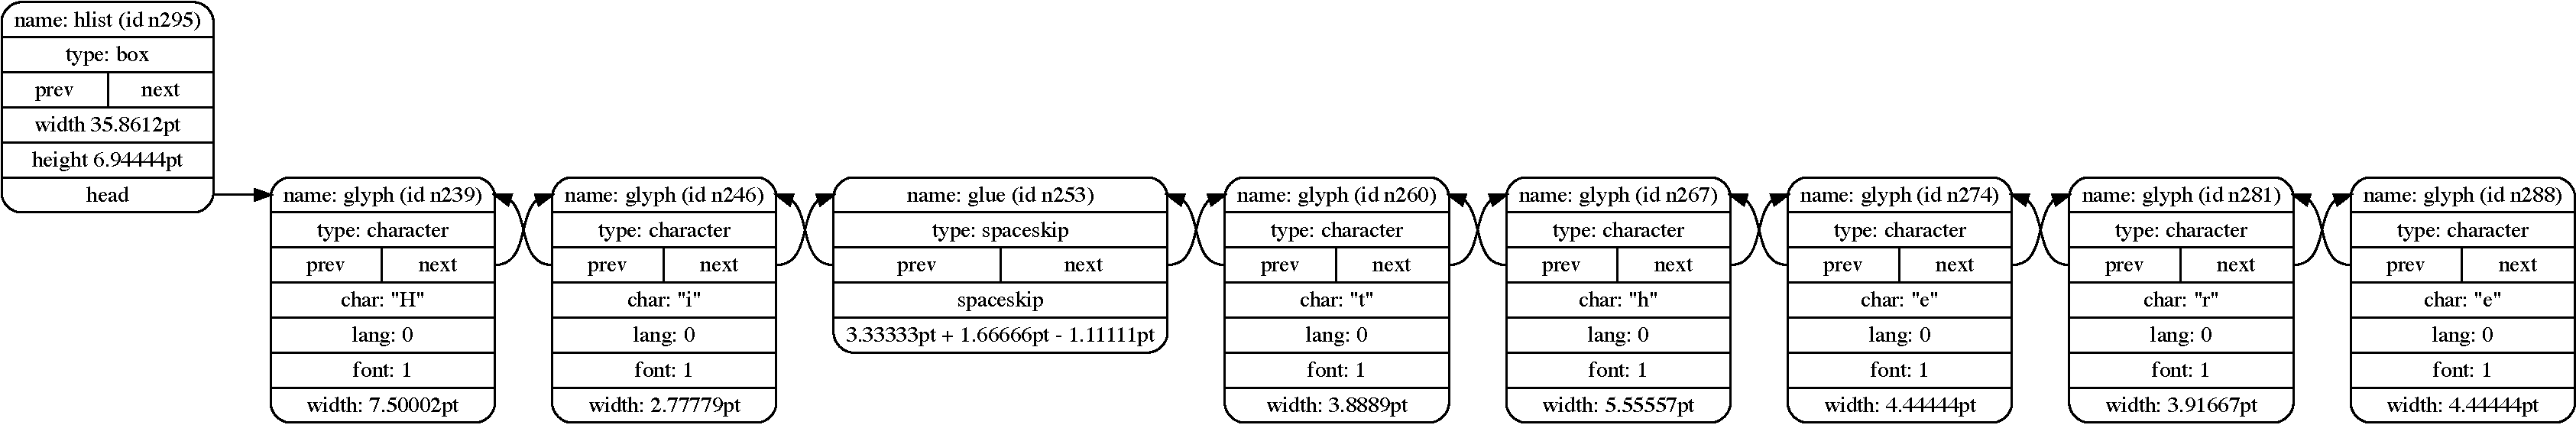
\includegraphics[width=4in]{hithere1.pdf}}

  \vglue-18.5mm
  \hbox{\hskip15mm \verb|\hbox{Hi there}|}

  \vglue 19.5mm
  \begin{minipage}{.5\textwidth}
    \begin{Verbatim}[fontsize=\small]
\hsize 90pt
A long time ago in a galaxy
far, far away $\ldots$.
\par
    \end{Verbatim}
  \end{minipage}
  \begin{minipage}{.35\textwidth}
    \fboxsep-\fboxrule
    \fbox{
\includegraphics[width=1.8in]{para.pdf}}
  \end{minipage}

  \hskip-2mm
  \href{run:images/nodelist.pdf}{
\includegraphics[width=4.4in]{nodelist.pdf}}
\end{frame}

\begin{frame}[fragile]{노드 리스트 순회 방법}
  노드 리스트 안의 노드들을 방문하면서 여러가지 일을 할 수 있다.

  포인터 \alert{head}로 노드 리스트의 첫번째 노드를
  알 수 있고, 그 노드의 \alert{next} 포인터를 따라가면
  다음 노드로 이동하고, 또 그 노드의 \alert{next} 포인터를 따라가고 $\ldots$.

  \begin{algorithm}[H]
    \SetAlgoNoLine
    \alert{
    노드\_포인터 := 리스트의 시작 노드\;
    \While{노드\_포인터가 nil 이 아니다}{
      노드\_포인터가 가리키는 노드를 방문한다\;
      노드\_포인터를 현재 노드의 next 포인터로 변경한다\;
    }}
  \end{algorithm}

  \href{run:images/hithere1.pdf}{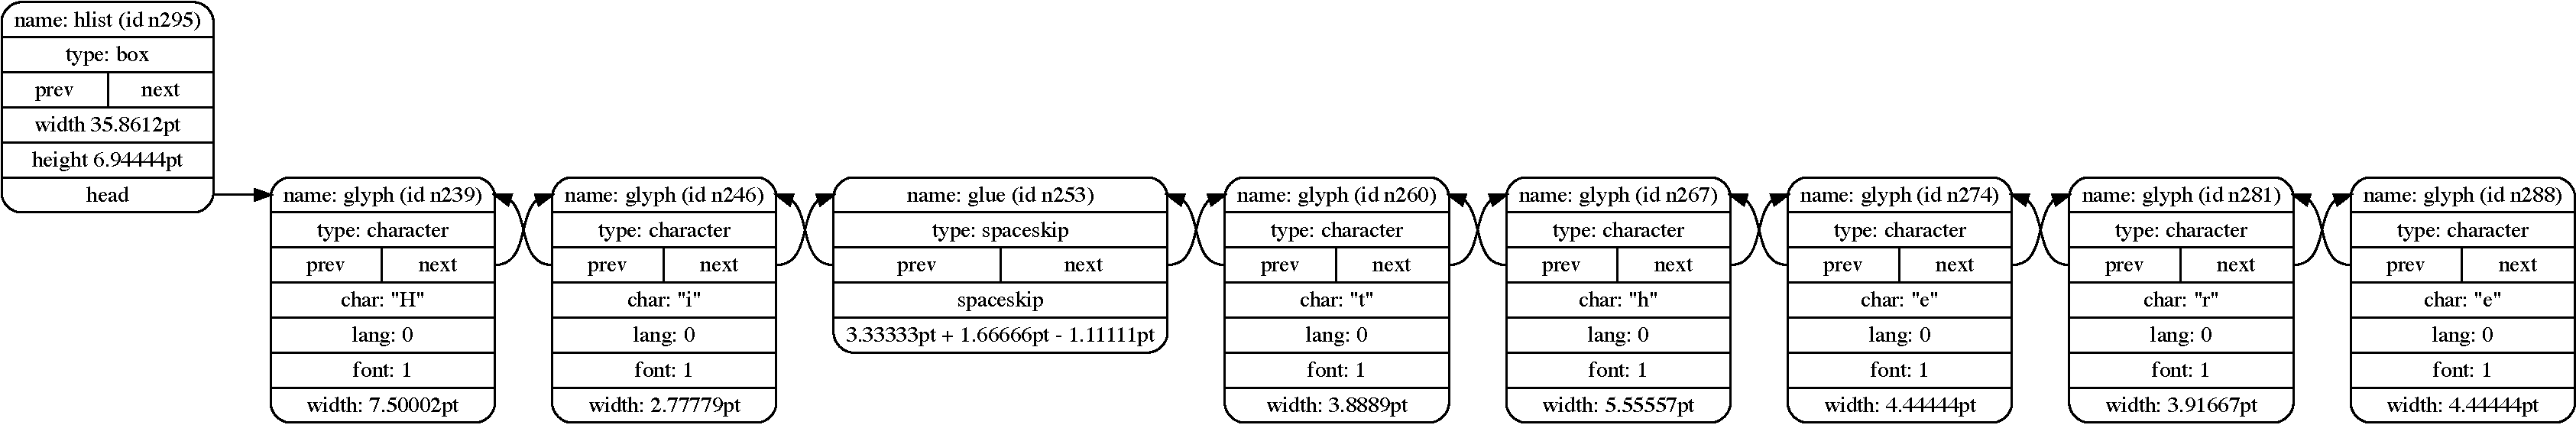
\includegraphics[width=4in]{hithere1.pdf}}

  \vglue-18.5mm
  \hbox{\hskip15mm \verb|\hbox{Hi there}|}
\end{frame}

\begin{frame}[fragile]{노드 리스트 순회 방법}
  \begin{algorithm}[H]
    \SetAlgoNoLine
    노드\_포인터 := 리스트의 시작 노드\;
    \While{노드\_포인터가 nil 이 아니다}{
      \alert{\If{노드\_포인터가 가리키는 노드가 hlist/vlist 노드 이다}{
        그 노드의 리스트를 순회 한다\;
      }}
      노드\_포인터가 가리키는 노드를 방문한다\;
      노드\_포인터를 현재 노드의 \alert{next} 포인터로 변경한다\;
    }
  \end{algorithm}

  \hskip-2mm
  \href{run:images/nodelist.pdf}{
\includegraphics[width=4.4in]{nodelist.pdf}}
\end{frame}

\begin{frame}[fragile]{노드 리스트 순회 방법}
  \begin{Verbatim}[fontsize=\small,commandchars=\\\{\}]
\alert{visit_node} = function (head)
   local curr = head
   while curr ~= nil do
      if curr.id == \alert{0} or curr.id == \alert{1} then \alert{-- hlist/vlist}
         \alert{visit_node}(curr.head)
      elseif curr.id == \alert{29} then  \alert{-- glyph}
         do_something_with_glyph(curr)
      elseif curr.id == \alert{12} then  \alert{-- glue}
         do_something_with_glue(curr)
      end
      curr = curr.next
   end
   return head
end
  \end{Verbatim}
\end{frame}

\begin{frame}[fragile]{노드 리스트 순회 방법}
  \begin{Verbatim}[fontsize=\small,commandchars=\\\{\}]
\href{https://github.com/sjnam/luatexko/blob/master/luatexko.lua\#L500-L555}{\alert{visit_node}} = function (head)
   local curr = head
   while curr ~= nil do
      if curr.id == \alert{node.id("hlist")}
         or curr.id == \alert{node.id("vlist")} then
         \alert{visit_node}(curr.head)
      elseif curr.id == \alert{node.id("glyph")} then
         do_something_with_glyph(curr)
      elseif curr.id == \alert{node.id("glue")} then
         do_something_with_glue(curr)
      end
      curr = curr.next
   end
   return head
end
  \end{Verbatim}
\end{frame}

\begin{frame}[fragile]{노드 리스트 순회 방법}
\begin{Verbatim}[fontsize=\small,commandchars=\\\{\}]
\alert{visit_glyph_node} = function (head)
   for curr in \alert{node.traverse_id(node.id("glyph"), head)} do
      do_something_with_glyph(curr)
   end
   return head
end
\end{Verbatim}

\begin{Verbatim}[fontsize=\small,commandchars=\\\{\}]
\alert{visit_hlist_node} = function (head)
   for curr in \alert{node.traverse_id(node.id("hlist"), head)} do
      do_something_with_hlist(curr)
   end
   return head
end
\end{Verbatim}
\end{frame}

\begin{frame}[fragile]{노드 라이브러리}
  노드 또는 노드 리스트를 쉽게 다룰 수 있도록 여러가지 유틸리티를 제공

\begin{Verbatim}[fontsize=\small]
  node.id(), node.new(), node.remove(),
  node.copy(), node.free(), node.flush_node(),
  node.traverse(), node.traverse_id(),
  node.traverse_char(), node.traverse_glyph(),
  node.traverse_list(), node.slide(),
  node.tail(),
  node.insert_before(), node.insert_after(),
  node.hpack(), node.vpack(),
  node.ligatureing(), node.kerning(),
  node.lastnode(),
  ...
\end{Verbatim}
\end{frame}

\section{콜백 Callbacks}

\begin{frame}[fragile]{콜백: 프로그래밍 관점에서}
  콜백은 함수인데 주로 다른 함수의 인수로 사용된다. 콜백을 넘겨받는 함수는
  특정 이벤트가 발생하거나 어떤 조건을 만족하면 콜백을 호출하여 실행한다.

  \textit{A nice way of imagining how a callback function works is that it is a
  function that is \alert{called at the back} of the function it is
  passed into.}

  \alert{훅(Hooks)}: 프로그램의 실행 흐름에서 특정 단계의 전, 후에 추가되거나
  그 단계를 대체하여 실행하는 코드(함수)에 관한 프로그래밍 기법이다.

  훅에서 실행되는 코드나 함수를 \alert{핸들러(handler)}라고 하고, 이때 사용되는
  개념이 콜백이다.

  핸들러를 특정 단계 전/후에 추가하거나 대체하는 과정을 "\alert{핸들러를
    등록(register)한다}" 라고 한다.
\end{frame}

\begin{frame}[fragile]{콜백: 루아텍 관점에서}
  루아텍의 콜백은 앞서 설명한 훅의 핸들러에 해당한다.

  텍 처리 과정인 \alert{입력, 확장, 실행, 조판}의 단계에서 원하는
  곳에 콜백을 등록하여 텍 동작을 수정하거나 갈아 치울 수 있다.

  \alert{\href{http://wiki.luatex.org/index.php/Callbacks}{콜백}}은
  텍이 입력 버퍼를 처리하는 데서 부터 문단을 만들거나 오프타입 폰트를 로딩하는
  부분까지 다양하다.

  \medskip
  콜백 등록과 해제

  \begin{Verbatim}[fontsize=\small]
my_cb = function (an_arg)
   do_something_with(an_arg)
end
callback.register("some_callback", my_cb)
callback.register("some_callback", nil)
  \end{Verbatim}
\end{frame}

\section{노드와 콜백 사용 예제}

\begin{frame}{Centred last lines}
  \begin{center}
    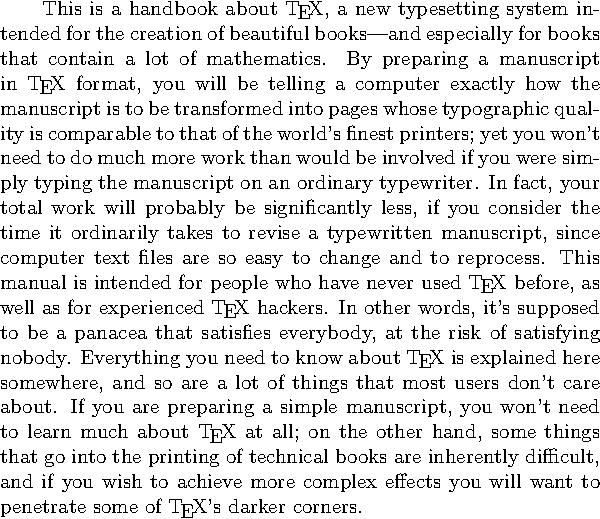
\includegraphics[width=3.2in]{lcenter0.pdf}
  \end{center}
\end{frame}

\begin{frame}{Centred last lines}
  \begin{center}
    
\includegraphics[width=3.2in]{lcenter.pdf}
  \end{center}
\end{frame}

\begin{frame}[fragile]{Centred last lines}
  \begin{Verbatim}[fontsize=\small,commandchars=\\\{\}]
\alert{centred_lastline} = function (head)
   local myglue = node.new(node.id("glue"))
   myglue.width = 0             \alert{-- 0pt plus 1fil}
   myglue.stretch = 1*2^16
   myglue.stretch_order = 2

   local line = node.tail(head) \alert{-- last line}
   node.insert_before(line.head, line.head, myglue)
   line.head = myglue

   line.head = node.hpack(line.head, line.width, "exactly")
   return head
end
luatexbase.add_to_callback(\alert{"post_linebreak_filter"},
                            centred_lastline,
                           "centred_lastline")
  \end{Verbatim}
\end{frame}

\begin{frame}[fragile]{Centred last lines}
  \alert{\TeX\ by Topic} 18.3.1 Centred last lines
  \begin{Verbatim}[fontsize=\small]
\leftskip=0cm plus 0.5fil \rightskip=0cm plus -0.5fil
\parfillskip=0cm plus 1fil
  \end{Verbatim}
\end{frame}

\begin{frame}[fragile]{Raggedright}
  \begin{center}
    
\includegraphics[width=3.3in]{victor_ragg.pdf}
  \end{center}
\end{frame}

\begin{frame}[fragile]{Justified}
  \begin{center}
    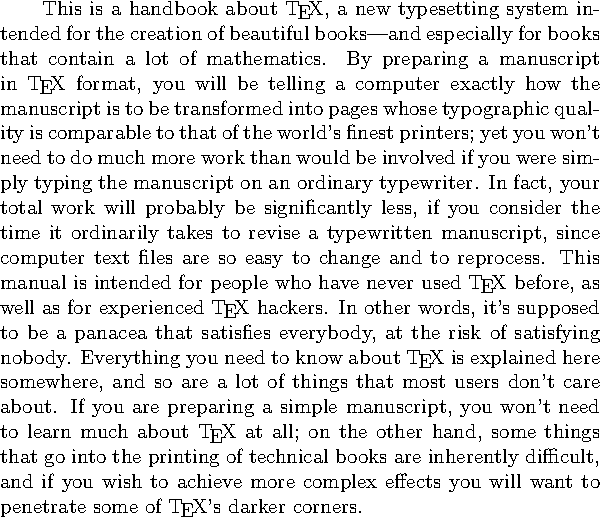
\includegraphics[width=3.2in]{victor_org.pdf}
  \end{center}
\end{frame}

\begin{frame}[fragile]{Between raggedright and justified}
  \begin{center}
    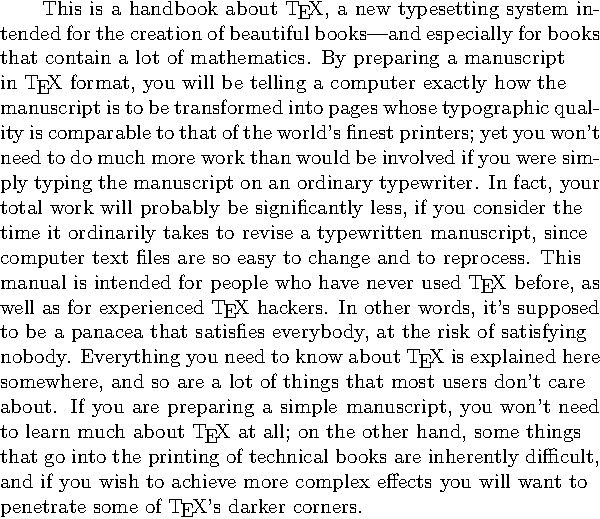
\includegraphics[width=3.2in]{victor.pdf}
  \end{center}
\end{frame}

\begin{frame}[fragile]{Between raggedright and justified}
  \begin{Verbatim}[fontsize=\small,commandchars=\\\{\}]
\alert{eatlines} = function (head)
   for line in node.traverse_id(node.id("hlist"), head) do
      if line.glue_order == 0    \alert{-- finite glue}
         and line.glue_sign == 1 \alert{-- stretching}
         and line.glue_set > .2  \alert{-- ratio}
      then
         line.head = node.hpack(line.head)
      end
   end
   return head
end
luatexbase.add_to_callback("post_linebreak_filter",
                            eatlines, "eatlines")
  \end{Verbatim}
\end{frame}

\begin{frame}[fragile]{Between raggedright and justified}
  \alert{\TeX\ by Topic} 5.9.6 Dissecting paragraphs with
  \texttt{\string\lastbox}
  \begin{Verbatim}[fontsize=\small,commandchars=+\[\]]
\newbox\linebox \newbox\snapbox
\def\eatlines{
  \setbox\linebox\lastbox    +alert[% check the last line]
  \ifvoid\linebox
  \else                      +alert[% if it's not empty]
  \unskip\unpenalty          +alert[% take whatever is]
  {\eatlines}                +alert[% above it;]
                             +alert[% collapse the line]
  \setbox\snapbox\hbox{\unhcopy\linebox}
                     +alert[% depending on the difference]
  \ifdim\wd\snapbox<.98\wd\linebox
        \box\snapbox +alert[% take the one ore the other,]
  \else \box\linebox \fi
  \fi}
  \end{Verbatim}
\end{frame}

\begin{frame}{Fadelines}
  \begin{center}
    
\includegraphics[width=3in]{fade.pdf}
  \end{center}
\end{frame}

\begin{frame}[fragile]{Fadelines}
  \begin{Verbatim}[fontsize=\small,commandchars=\\\{\}]
\alert{fadelines} = function (head)
   local graycolor = node.new("whatsit", "pdf_colorstack")
   local gvalue = 0
   for line in node.traverse_id(node.id("hlist"), head) do
      graycolor.data = gvalue .. " g"
      node.insert_before(head, line, node.copy(graycolor))
      gvalue = math.min(gvalue+0.06, 1)
   end
   return head
end
luatexbase.add_to_callback("post_linebreak_filter",
                            fadelines, "fadelines")
  \end{Verbatim}
\end{frame}

\chickenizesetup{
  rainbow_step=0.3
}
\let\tempone\itemize
\let\temptwo\enditemize
\renewenvironment{itemize}{\tempone\addtolength{\itemsep}{0.5\baselineskip}}
                 {\temptwo}
\begin{frame}[fragile]{다양한 예제}
  \begin{itemize}
  \item {\rainbowcolor\fontspec[Scale=1.5,Letters=Random]{Punk Nova}
    chickenize\par\unrainbowcolor}
  \item \href{https://www.tug.org/TUGboat/tb31-3/tb99isambert.pdf}%
    {\alert{Three things you can do with Lua\TeX\ that would be extremely %
        painful otherwise}}
  \item \href{https://gist.github.com/dohyunkim/cde58679facb606a01a9\#file-drawcharbox-lua-L56-L77}%
    {gist.github.com/dohyunkim/drawcharbox.lua}
  \item \href{https://github.com/dohyunkim/colorjamo/blob/master/colorjamo.lua\#L110-L138}%
    {github.com/dohyunkim/colorjamo}
  \item \href{https://github.com/dohyunkim/luatexko}%
    {github.com/dohyunkim/luatexko}
  \item \href{https://tex.stackexchange.com/search?q=\%5Bluatex\%5D+callback}%
    {https://tex.stackexchange.com/search?q=\%5Bluatex\%5D+callback}
  \end{itemize}
\end{frame}

\section{맺음말}

\begin{frame}[fragile]{Lua\TeX nician이 되는 방법}
  간단하다. 아래의 책들을 순서대로 읽는다.
  \begin{enumerate}
  \item \alert{The \TeX book} by Donald E. Knuth
  \item \alert{\TeX\ by Topic, A \TeX nician's Reference} by Victor Eijkhout
  \item \alert{The $\varepsilon$-\TeX\ manual} by The NTS Team
  \item \alert{The pdf\TeX\ user manual} by Han The Thanh and friends
  \item \alert{Programming in Lua} by Roberto Ierusalimschy
  \item \alert{The Lua\TeX\ Reference Manual} by Lua\TeX\ deveopment team
  \end{enumerate}

  루아테크니션이 되었다면, \alert{\href{http://github.com/dohyun/luatexko}%
  {Lua\TeX-ko 개발}}에 참여한다.
\end{frame}

\begin{frame}{맺음말}
  \begin{itemize}
  \item 루아텍은 노드와 콜백으로 그동안 다루기 힘들었던 텍 내부에 접근 할 수
    있게 되었다.
  \item 루아텍을 통하여 텍의 진수를 맛볼  수 있다.
  \item 패키지 개발할때 루아텍을 이용하는 것이 더욱 직관적이고 코드도 이해하기
    쉽고, 버그를 줄일 수 있다.
  \item 루아텍은 패키지 개발자 뿐만 아니라, 일반 사용자에게도 많은 이로움을
    제공한다. 특히 한글 문서는 Lua\TeX-ko를 사용하는 것을 권한다.
  \item 일반 (라)텍 사용자를 넘어 루아테크니션이 되자.
  \end{itemize}
\end{frame}

\end{document}
